\documentclass{article}
\usepackage[T1]{fontenc}
\usepackage{lmodern}
\usepackage{amsmath}
\usepackage{graphicx}
\usepackage{float}
\usepackage{listings}
\usepackage{xcolor}
\usepackage[polish]{babel}

\usepackage[a4paper, margin=2.54cm]{geometry}

\title{Praca domowa 2\\Metoda gradientowa oraz\\
minimalizacja wybranej funkcji}
\author{Damian Jankowski s188597}

\begin{document}

\maketitle

\section{Wstęp}
Tematem pracy domowej jest zapoznanie się z minimalizacją funkcji
metodą gradientową. W tym celu wybrałem funkcję
$f(x, y) = 3(x-1)^2-2(x-1)y+3y^2$. Minimum funkcji to $f(1, 0) = 0$.

Poszukiwanie minimum funkcji
zaczęłem od wybrania losowego punktu startowego $X_0$ z zakresu
$-3 \le x \le 3$ oraz $-3 \le y \le 3$.

\begin{figure}[H]
    \centering
    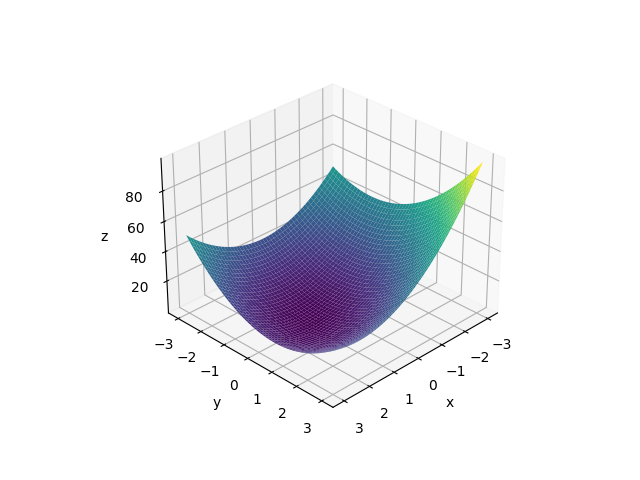
\includegraphics[width=0.5\textwidth]{function.png}
    \caption{Wykres funkcji $f(x, y)$}
\end{figure}


\section{Zadanie}
Do wyznaczenia minimum funkcji metodą gradientową trzeba użyć
wzoru:
\begin{equation}
X_{k+1} = X_k - \alpha_k \nabla f(X_k)
\end{equation}
gdzie $\alpha_k$ jest stałą kroku, 
a $\nabla f(X_k)$ jest gradientem
funkcji $f(x, y)$ w punkcie $X_k$.

Gradient funkcji $f(x, y)$ to inaczej wektor pochodnych
cząstkowych:
\begin{equation}
\nabla f(x, y) = \left( \frac{\partial f}{\partial x}, \frac{\partial f}{\partial y} \right)
\end{equation}
W przypadku wybranej funkcji gradient ma postać:
\begin{equation}
\nabla f(x, y) = {6(x - 1)-2y \choose -2(x-1)+6y}
\end{equation}
Dla tego przykładu stała kroku $\alpha_k = 0.1$ natomiast
warunek zakończenia to wartość funkcji mniejsza niż $10^{-4}$ lub 
ilość iteracji większa niż 1000.

\section{Przykładowe obliczenia}

Dla przykładowego punktu startowego $X_0 = (-2, 3)$
wyznaczenie 5 kolejnych punktów wygląda następująco:
\begin{equation*}
    \begin{aligned}
    X_1 &= {{-2} \choose {3}} - 0.1 {6(-2 - 1)-2\cdot3 \choose -2\cdot(-2-1)+6\cdot3} = {{0.4} \choose {0.6}} \\
    X_2 &= {{0.4} \choose {0.6}} - 0.1 {6(0.4 - 1)-2\cdot0.6 \choose -2\cdot(0.4-1)+6\cdot0.6} = {{0.88} \choose {0.12}} \\
    X_3 &= {{0.88} \choose {0.12}} - 0.1 {6(0.88 - 1)-2\cdot0.12 \choose -2\cdot(0.88-1)+6\cdot0.12} = {{0.976} \choose {0.024}} \\
    X_4 &= {{0.976} \choose {0.024}} - 0.1 {6(0.976 - 1)-2\cdot0.024 \choose -2\cdot(0.976-1)+6\cdot0.024} = {{0.9952} \choose {0.0048}} \\
    X_5 &= {{0.9952} \choose {0.0048}} - 0.1 {6(0.9952 - 1)-2\cdot0.0048 \choose -2\cdot(0.9952-1)+6\cdot0.0048} = {{0.99904} \choose {0.00096}}
    \end{aligned}
\end{equation*}

Dla tego przykładu wartość funkcji w punkcie $X_5$ wynosi $f(X_5) = 7.3727 \cdot 10^{-6}$,
algorytm się kończy.

\begin{figure}[H]
    \centering
    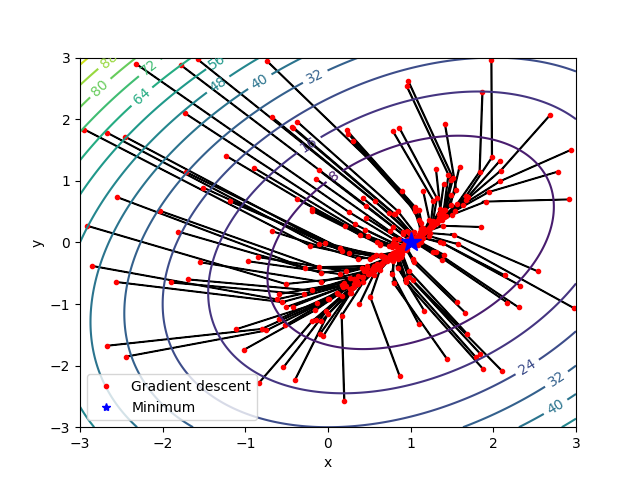
\includegraphics[width=0.5\textwidth]{plot.png}
    \caption{Rzut 2D funkcji $f(x, y)$ oraz kolejne kroki
    minimalizacji metodą gradientową} {dla wylosowanych 100 punktów startowych}
\end{figure}

Po wykonaniu obliczeń dla 100 losowo wybranych
punktów startowych średnia wartość
iteracji do osiągnięcia minimum wynosiła około 10.

\section{Wnioski}
Metoda gradientowa jest efektywną metodą szukania minimum funkcji, 
która polega na iteracyjnym kroku w kierunku przeciwnym do gradientu 
funkcji w danym punkcie. Metoda ta wymaga znajomości pochodnych 
cząstkowych funkcji, co może być trudne lub czasochłonne dla bardziej 
skomplikowanych funkcji.

W przypadku funkcji o jednym minimum globalnym, metoda gradientowa 
zwykle osiąga minimum w niewielkiej liczbie kroków. Jednak w przypadku 
funkcji z wieloma minimami lokalnymi, metoda ta może "utknąć" w minimum 
lokalnym i nie osiągnąć minimum globalnego.

\section{Kod programu}
\lstinputlisting[
language=python,  
basicstyle=\small\tt,
keywordstyle=\color{blue},
backgroundcolor=\color{cyan!10}
]{main.py}

\end{document}
